%%%%%%%%%%%%%%%%%%%%%%%%%%%%%%%%%%%%%%%%%
% Beamer Presentation
% LaTeX Template
% Version 1.0 (10/11/12)
%
% This template has been downloaded from:
% http://www.LaTeXTemplates.com
%
% License:
% CC BY-NC-SA 3.0 (http://creativecommons.org/licenses/by-nc-sa/3.0/)
%
%%%%%%%%%%%%%%%%%%%%%%%%%%%%%%%%%%%%%%%%%

%----------------------------------------------------------------------------------------
%	PACKAGES AND THEMES
%----------------------------------------------------------------------------------------

\documentclass{beamer}

\mode<presentation> {

% The Beamer class comes with a number of default slide themes
% which change the colors and layouts of slides. Below this is a list
% of all the themes, uncomment each in turn to see what they look like.

%\usetheme{default}
%\usetheme{AnnArbor}
%\usetheme{Antibes}
%\usetheme{Bergen}
\usetheme{Berkeley}
%\usetheme{Berlin}
%\usetheme{Boadilla}
%\usetheme{CambridgeUS}
%\usetheme{Copenhagen}
%\usetheme{Darmstadt}
%\usetheme{Dresden}
%\usetheme{Frankfurt}
%\usetheme{Goettingen}
%\usetheme{Hannover}
%\usetheme{Ilmenau}
%\usetheme{JuanLesPins}
%\usetheme{Luebeck}
%\usetheme{Madrid}
%\usetheme{Malmoe}
%\usetheme{Marburg}
%\usetheme{Montpellier}
%\usetheme{PaloAlto}
%\usetheme{Pittsburgh}
%\usetheme{Rochester}
%\usetheme{Singapore}
%\usetheme{Szeged}
%\usetheme{Warsaw}

% As well as themes, the Beamer class has a number of color themes
% for any slide theme. Uncomment each of these in turn to see how it
% changes the colors of your current slide theme.

%\usecolortheme{albatross}
%\usecolortheme{beaver}
%\usecolortheme{beetle}
%\usecolortheme{crane}
\usecolortheme{dolphin}
%\usecolortheme{dove}
%\usecolortheme{fly}
%\usecolortheme{lily}
%\usecolortheme{orchid}
%\usecolortheme{rose}
%\usecolortheme{seagull}
%\usecolortheme{seahorse}
%\usecolortheme{whale}
%\usecolortheme{wolverine}

%\setbeamertemplate{footline} % To remove the footer line in all slides uncomment this line
%\setbeamertemplate{footline}[page number] % To replace the footer line in all slides with a simple slide count uncomment this line

%\setbeamertemplate{navigation symbols}{} % To remove the navigation symbols from the bottom of all slides uncomment this line
}

\usepackage{graphicx} % Allows including images
\usepackage{booktabs} % Allows the use of \toprule, \midrule and \bottomrule in tables
\usepackage[utf8]{inputenc}
\usepackage{multirow}

%----------------------------------------------------------------------------------------
%	TITLE PAGE
%----------------------------------------------------------------------------------------

\title[EP1]{EP1 - MAC0422} % The short title appears at the bottom of every slide, the full title is only on the title page

\author{João Gabriel e Juliano Garcia} % Your name
\institute[IME- USP] % Your institution as it will appear on the bottom of every slide, may be shorthand to save space
{
Instituto de Matemática e Estatística - USP \\ % Your institution for the title page
}
\date{} % Date, can be changed to a custom date

\begin{document}

\begin{frame}
\titlepage % Print the title page as the first slide
\end{frame}

\begin{frame}
\frametitle{Overview} % Table of contents slide, comment this block out to remove it
\tableofcontents % Throughout your presentation, if you choose to use \section{} and \subsection{} commands, these will automatically be printed on this slide as an overview of your presentation
\end{frame}

%----------------------------------------------------------------------------------------
%	PRESENTATION SLIDES
%----------------------------------------------------------------------------------------

%------------------------------------------------
\section{Shell}
%------------------------------------------------

\begin{frame}
\begin{center}
\huge Shell
\end{center}
\end{frame}

\begin{frame}
\frametitle{Estruturas de dados utilizadas}
\begin{itemize}
\item Buffer de caracteres (buffer.h): Para ler a linha de comando
\item Módulo de erros (error.h): Para tratar erros gerados por funções de bibliotecas externas
\item pid\_t (sys/types.h): Estrutura padrão do "sys/types" para armazenar PID de processos
\end{itemize}
\end{frame}

\begin{frame}
\frametitle{Decisões de projeto}
\begin{itemize}
\item A shell obtém o PATH do sistema, assim ela pode executar programas sem que seja especificado todo o caminho, desde a pasta root
\item Além dos comandos "chown" e "date" há um terceiro comando implementado por nós: o "exit". Ele termina a execução da shell, desalocando todas as estruturas alocadas por ela
\item Para executar outros comandos, o programa executa um "fork", criando assim um processo filho, e utiliza "execvp" no processo filho para executar o programa solicitado e "waitpid" no processo pai (a shell) para que ela espere o filho acabar de executar
\end{itemize}
\end{frame}

%------------------------------------------------

% Blocks:
%\begin{block}{Block 1}
%Lorem ipsum dolor sit amet, consectetur adipiscing elit. Integer lectus nisl, ultricies in feugiat rutrum, porttitor sit amet augue. Aliquam ut tortor mauris. Sed volutpat ante purus, quis accumsan dolor.
%\end{block}

% Paragraph division: \\~\\

% Columns
%\begin{columns}[c] % The "c" option specifies centered vertical alignment while the "t" option is used for top vertical alignment

%\column{.45\textwidth} % Left column and width
%\textbf{Heading}
%\begin{enumerate}
%\item Statement
%\item Explanation
%\item Example
%\end{enumerate}

%\column{.5\textwidth} % Right column and width
%Lorem ipsum dolor sit amet, consectetur adipiscing elit. Integer lectus nisl, ultricies in feugiat rutrum, porttitor sit amet augue. Aliquam ut tortor mauris. Sed volutpat ante purus, quis accumsan dolor.

%\end{columns}

%------------------------------------------------
\section{Simulador de processos}
%------------------------------------------------

\begin{frame}
\begin{center}
\huge Simulador de processos
\end{center}
\end{frame}

\begin{frame}
\frametitle{Estruturas de dados}
\begin{itemize}
\item Fila de prioridade (minPQ.h): Para ordenar os processos no SJF
\item Fila (queue.h): Para a fila de processos no Round Robin e no escalonador com prioridade
\item Pilha (stack.h): Para guardar os processos que ainda não chegaram
\item Process (process.h): Para armazenar todas as informações sobre um processo
\item Timer (time.h): Para cronometrar os tempos
\end{itemize}
\end{frame}

\begin{frame}
\frametitle{Threads}
\begin{itemize}
\item Todos os escalonadores são multithreaded
\item A quantidade de processos simulados paralelamente é a quantidade de CPUs da máquina que está rodando o programa
\item Usamos mutexes para as seções críticas de cada thread e do próprio escalonador
\item Variáveis de condição: A thread do escalonador é bloqueada até que receba um sinal de algum processo que terminou o seu "turno"
\item Para simular as CPUs, implementamos uma lista, onde cada posição representa uma CPU. A posição é marcada com 1 se a CPU está sendo usada, ou 0 caso contrário
\end{itemize}
\end{frame}


\subsection{Shortest job first}

\begin{frame}
\frametitle{Loop do escalonador}
\begin{itemize}
\item Pilha de processos a serem executados
\item Processos que chegam são inseridos na fila de prioridade, ordenados por dt
\item A medida que há CPUs livres, processos são colocados para rodar paralelamente
\item Escalonador não prossegue a execução enquanto não houver CPU livre
\item Tirando a principal (escalonador), temos X threads para os processos, onde X é a quantidade de CPUs da máquina que roda um processo
\end{itemize}
\end{frame}

\begin{frame}
\frametitle{Visualização}
\begin{figure}
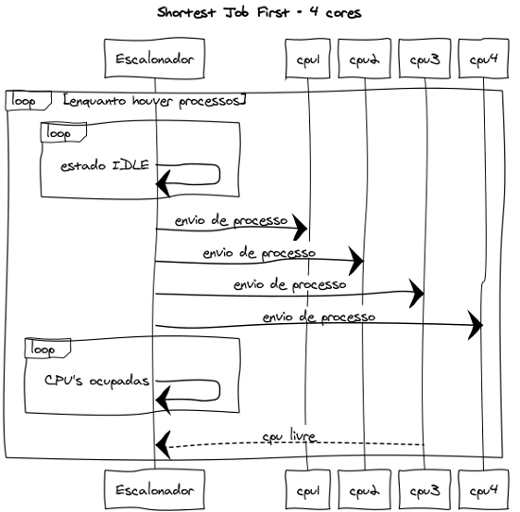
\includegraphics[scale=0.4]{sjf.png}
\end{figure}
\end{frame}

\begin{frame}
\frametitle{Estatísticas sobre cumprimento das deadlines}
\begin{table}
\begin{tabular}{l l l l l}
\toprule
\textbf{Cores} & \textbf{Arquivo} & \textbf{Média} & \textbf{Variância} & \textbf{IC}\\
\midrule
\multirow{3}{*}{32} & Pequeno & 100   & 0      & [100, 100] \\
					& Médio   & 100   & 0      & [100, 100] \\
					& Grande  & 100   & 0      & [100, 100] \\
\midrule
\multirow{3}{*}{4}  & Pequeno & 98.57 & 33.08  & [93.43, 100] \\
					& Médio   & 90.35 & 47.93  & [87.77, 92.93] \\
					& Grande  & 53.55 & 129.92 & [49.30, 57.80] \\
\bottomrule
\end{tabular}
\end{table}
\end{frame}

\begin{frame}
\frametitle{Estatísticas sobre mudanças de contexto}
\begin{table}
\begin{tabular}{l l l l l}
\toprule
\textbf{Cores} & \textbf{Arquivo} & \textbf{Média} & \textbf{Variância} & \textbf{IC}\\
\midrule
\multirow{3}{*}{32} & Pequeno & 0 & 0 & [0, 0] \\
					& Médio   & 0 & 0 & [0, 0] \\
					& Grande  & 0 & 0 & [0, 0] \\
\midrule
\multirow{3}{*}{4}  & Pequeno & 0 & 0 & [0, 0] \\
					& Médio   & 0 & 0 & [0, 0] \\
					& Grande  & 0 & 0 & [0, 0] \\
\bottomrule
\end{tabular}
\end{table}
\end{frame}

\subsection{Round Robin}

\begin{frame}
\frametitle{Loop do escalonador}
\begin{itemize}
\item Pilha de processos
\item Processos que chegam são adicionados em uma fila e é criado uma thread para cada processo
\item Se algum processo terminou de rodar, o escalonador o coloca de volta na fila
\item Se tem alguma CPU livre, e há processos na fila, o escalonador os coloca para rodar nas CPUs livres e os retira da fila
\item Depois de rodar por no máximo 1s, o processo sinaliza que acabou para o escalonador por meio de semáforos, e o escalonador volta para o começo do loop
\end{itemize}
\end{frame}

\begin{frame}
\frametitle{Visualização}
\begin{figure}
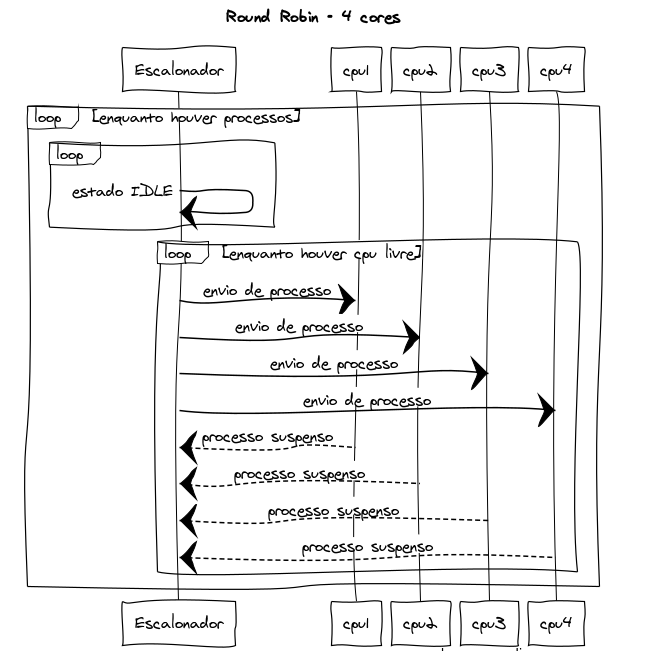
\includegraphics[scale=0.32]{rr.png}
\end{figure}
\end{frame}

\begin{frame}
\frametitle{Estatísticas sobre cumprimento das deadlines}
\begin{table}
\begin{tabular}{l l l l l}
\toprule
\textbf{Cores} & \textbf{Arquivo} & \textbf{Média} & \textbf{Variância} & \textbf{IC}\\
\midrule
\multirow{3}{*}{32} & Pequeno & 99.52 & 6.81   & [98.55, 100] \\
					& Médio   & 100   & 0      & [100, 100] \\
					& Grande  & 99.93 & 0.15   & [99.78, 100] \\
\midrule
\multirow{3}{*}{4}  & Pequeno & 98.57 & 19.01  & [96.95, 100] \\
					& Médio   & 62.81 & 257.77 & [56.82, 68.79] \\
					& Grande  & 2.34  & 13.84  & [0.95, 3.73] \\
\bottomrule
\end{tabular}
\end{table}
\end{frame}

\begin{frame}
\frametitle{Estatísticas sobre mudanças de contexto}
\begin{table}
\begin{tabular}{l l l l l}
\toprule
\textbf{Cores} & \textbf{Arquivo} & \textbf{Média} & \textbf{Variância} & \textbf{IC}\\
\midrule
\multirow{3}{*}{32} & Pequeno & 25.8   & 55.48    & [23.02, 28.58] \\
					& Médio   & 288.30 & 16380.15 & [240.59, 336.01] \\
					& Grande  & 600.03 & 58940.38 & [509.52, 690.54] \\
\midrule
\multirow{3}{*}{4}  & Pequeno & 25.8   & 55.48    & [23.02, 28.58] \\
					& Médio   & 288.30 & 16380.15 & [240.59, 336.01] \\
					& Grande  & 600.03 & 58940.38 & [509.52, 690.54] \\
\bottomrule
\end{tabular}
\end{table}
\end{frame}

\subsection{Escalonamento com prioridade}

\begin{frame}
\frametitle{Loop do escalonador}
\begin{itemize}
\item Pilha de processos
\item Processos que chegam são adicionados em uma fila, é criado uma thread para cada processo e é calculada sua prioridade
\item Se algum processo terminou de rodar, o escalonador ou o coloca de volta na fila, se ele precisar rodar mais, ou não coloca, caso contrário
\item Se tem alguma CPU livre, e há processos na fila, o escalonador os coloca para rodar nas CPUs livres e os retira da fila
\item O número de quanta que o processo irá rodar depende de sua prioridade e das prioridades dos outros processos que estão na fila ou nas CPUs
\end{itemize}
\end{frame}

\begin{frame}
\frametitle{Loop do escalonador}
\begin{itemize}
\item Depois de rodar por no máximo o seu número de quanta, o processo sinaliza que acabou para o escalonador por meio de semáforos, e o escalonador volta para o começo do loop
\end{itemize}
\end{frame}

\begin{frame}
\frametitle{Visualização}
\begin{figure}
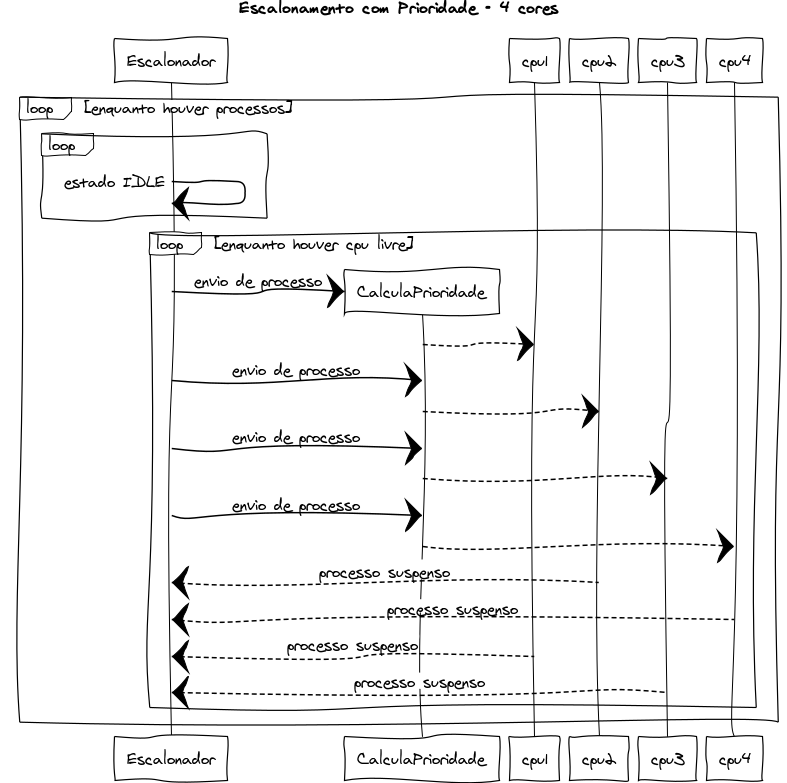
\includegraphics[scale=0.27]{prr.png}
\end{figure}
\end{frame}

\begin{frame}
\frametitle{C\'alculo da prioridade}
A prioridade de cada processo é definida de acordo com seus t0, dt e deadline usando a seguinte fórmula:
$$P(t_0, dt, punc) = a\cdot punc^2 + b\cdot punc + c\cdot dt + d\cdot t_0$$
Onde $punc = deadline - dt$, e os parâmetros são:
$$a=0.00213475762298$$
$$b=2.06241892813$$
$$c=0.21137699282$$
$$d=0.207715732988$$
Os parâmetros foram aprendidos usando gradiente descendente de acordo com algumas configurações de prioridade que nós estipulamos.
\end{frame}

\begin{frame}
\frametitle{Gráfico da prioridade}
\begin{figure}
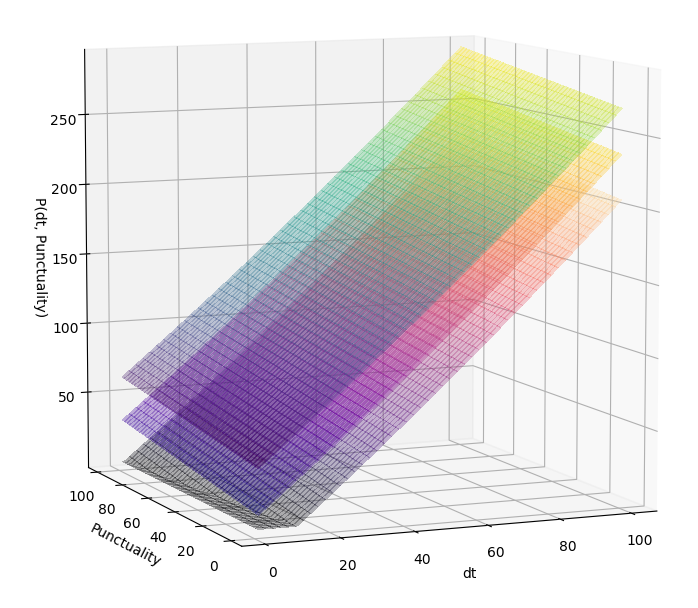
\includegraphics[width=0.8\linewidth]{pfunction.png}
\end{figure}
%???Gáfico???
\end{frame}

\begin{frame}
\frametitle{Cálculo do quanta}
O tempo máximo de execução de um processo é calculado a cada vez que esse processo (com prioridade p) sai da fila, usando a seguinte fórmula:
$$Q(p) = 1 + min\left\{2.25\cdot\frac{|p-\mu|}{\sigma},\quad 9\right\}$$
Onde:
\begin{itemize}
\item p: prioridade do processo atual
\item $\mu$: média das prioridades dos processos ativos (incluindo os da fila)
\item $\sigma$: desvio padrão das prioridades dos processos ativos (incluindo os da fila)
\end{itemize}
Essa fórmula garante que os processos com prioridades parecidas com a média tenham tempos pequenos e limita os tempos para o intervalo [1, 10]
\end{frame}

\begin{frame}
\frametitle{Estatísticas sobre cumprimento das deadlines}
\begin{table}
\begin{tabular}{l l l l l}
\toprule
\textbf{Cores} & \textbf{Arquivo} & \textbf{Média} & \textbf{Variância} & \textbf{IC}\\
\midrule
\multirow{3}{*}{32} & Pequeno & 97.14 & 47.83  & [94.53, 99.72] \\
 					& Médio   & 100   & 0      & [100, 100] \\
 					& Grande  & 99.93 & 0.15   & [99.78, 100] \\
\midrule
\multirow{3}{*}{4}  & Pequeno & 94.76 & 77.19  & [91.49, 98.04] \\
 					& Médio   & 60    & 348.82 & [53.04, 66.96] \\
 					& Grande  & 8.8   & 14.58  & [7.37, 10.22] \\
\bottomrule
\end{tabular}
\end{table}
\end{frame}

\begin{frame}
\frametitle{Estatísticas sobre mudanças de contexto}
\begin{table}
\begin{tabular}{l l l l l}
\toprule
\textbf{Cores} & \textbf{Arquivo} & \textbf{Média} & \textbf{Variância} & \textbf{IC}\\
\midrule
\multirow{3}{*}{32} & Pequeno & 8.63   & 12.03   & [7.34, 9.93] \\
					& Médio   & 118.47 & 3313.91 & [97, 139.93] \\
					& Grande  & 238.83 & 9929.94 & [201.68, 275.98] \\
\midrule
\multirow{3}{*}{4}  & Pequeno & 8.6    & 11.14   & [7.36, 9.84] \\
					& Médio   & 103.33 & 2278.57 & [85.54, 121.13] \\
					& Grande  & 206.63 & 7557.21 & [174.22, 239.04] \\
\bottomrule
\end{tabular}
\end{table}
\end{frame}
%------------------------------------------------
\section{Gráficos}
%------------------------------------------------

\begin{frame}
\begin{center}
\huge Gráficos
\end{center}
\end{frame}

\begin{frame}
\frametitle{Gerador de arquivos de trace}
\begin{figure}
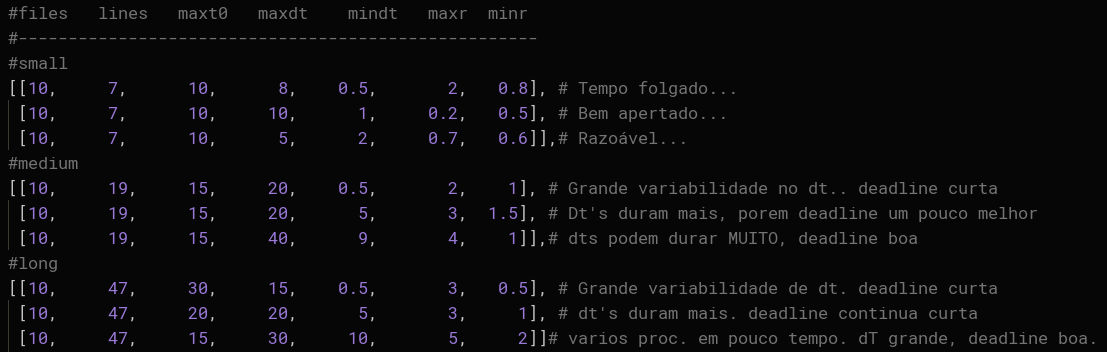
\includegraphics[scale=0.3]{trace_dist.png}
\end{figure}
\end{frame}


\subsection{Máquina A}

\begin{frame}
\frametitle{Cumprimento de deadlines (4 cores)}
\begin{figure}
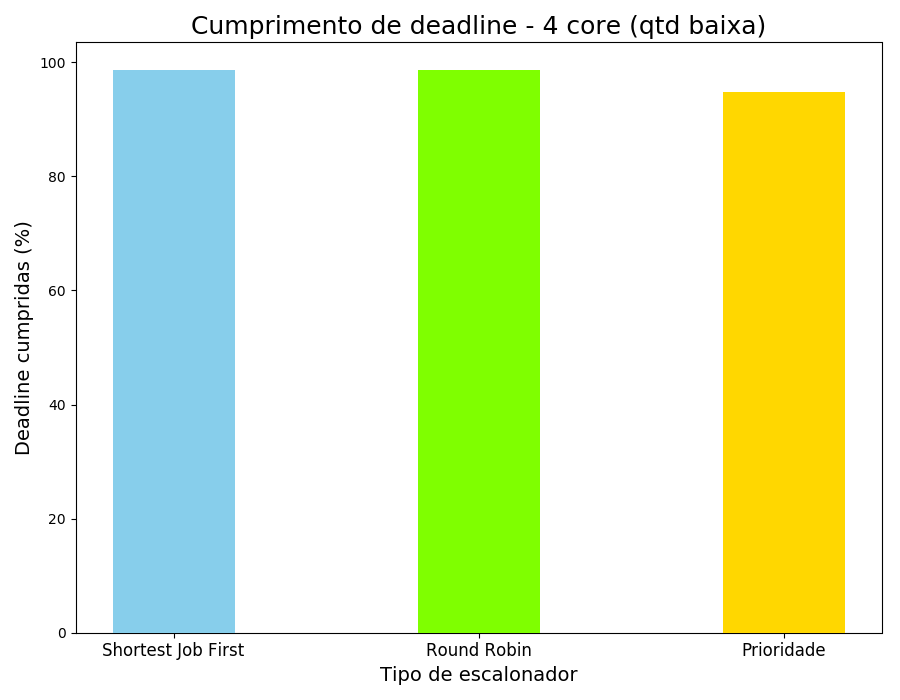
\includegraphics[scale=0.4]{deadline_small_4.png}
\end{figure}
\end{frame}

\begin{frame}
\frametitle{Cumprimento de deadlines (4 cores)}
\begin{figure}
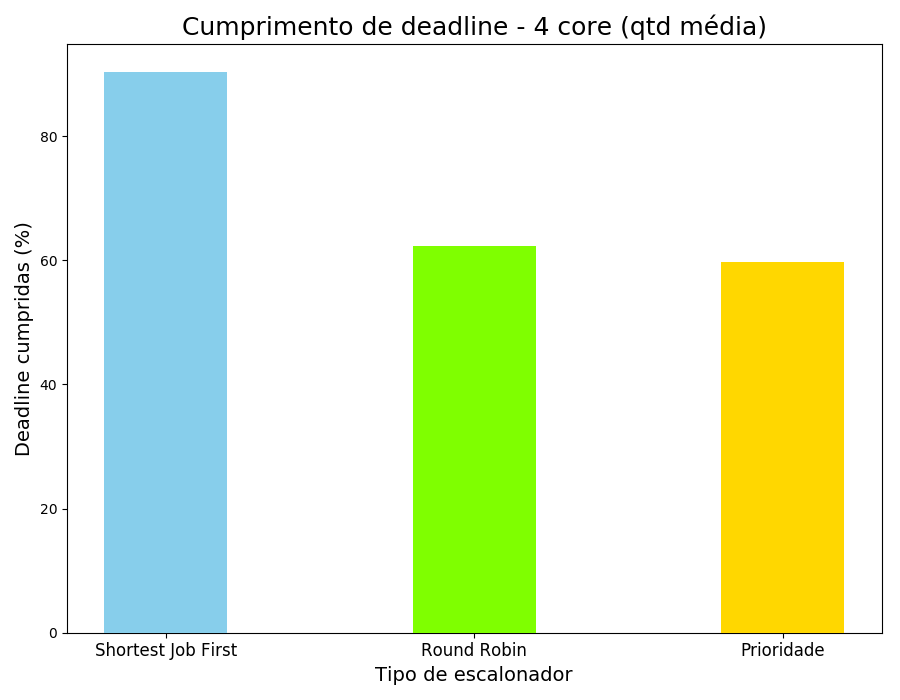
\includegraphics[scale=0.4]{deadline_med_4.png}
\end{figure}
\end{frame}

\begin{frame}
\frametitle{Cumprimento de deadlines (4 cores)}
\begin{figure}
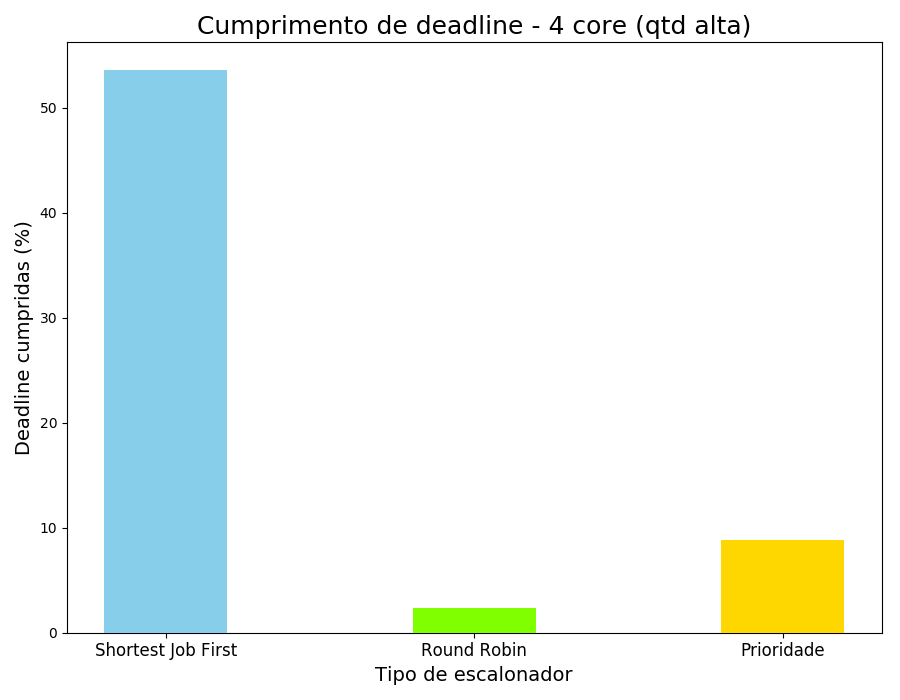
\includegraphics[scale=0.4]{deadline_long_4.png}
\end{figure}
\end{frame}

\begin{frame}
\frametitle{Mudanças de contexto (4 cores)}
\begin{figure}
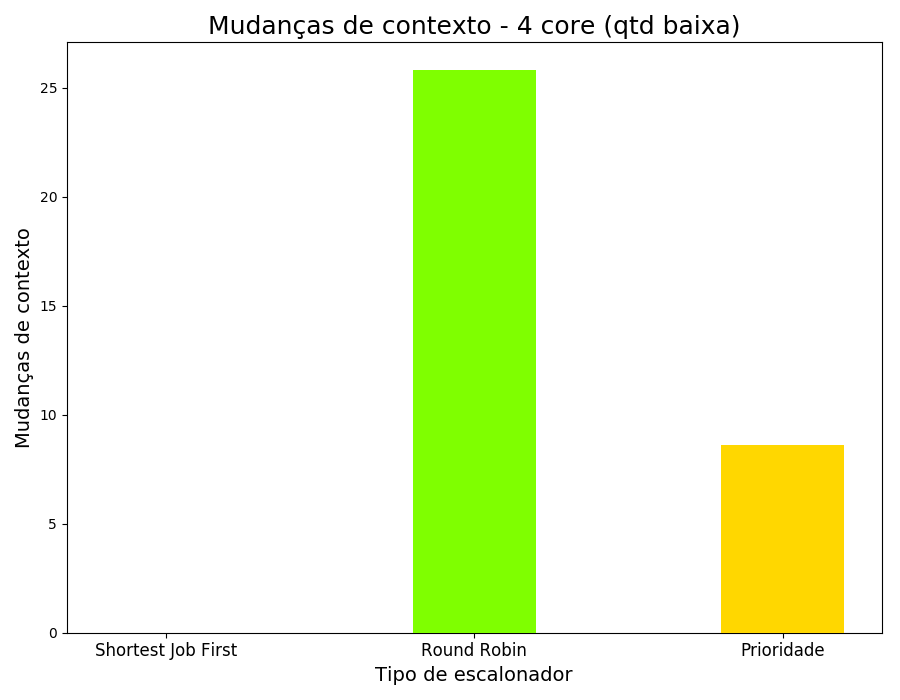
\includegraphics[scale=0.4]{ctx_small_4.png}
\end{figure}
\end{frame}

\begin{frame}
\frametitle{Mudanças de contexto (4 cores)}
\begin{figure}
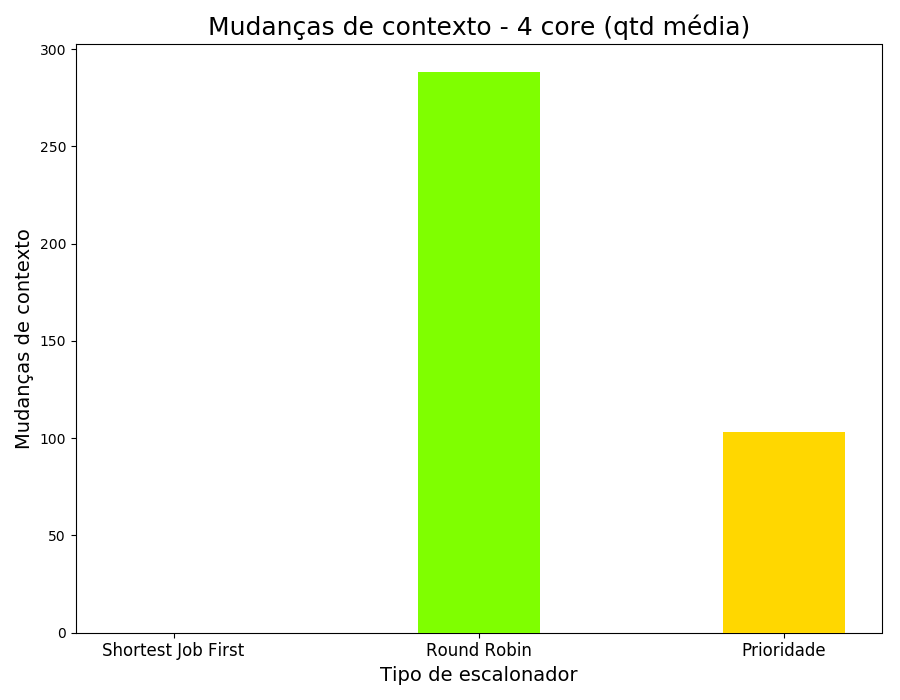
\includegraphics[scale=0.4]{ctx_med_4.png}
\end{figure}
\end{frame}

\begin{frame}
\frametitle{Mudanças de contexto (4 cores)}
\begin{figure}
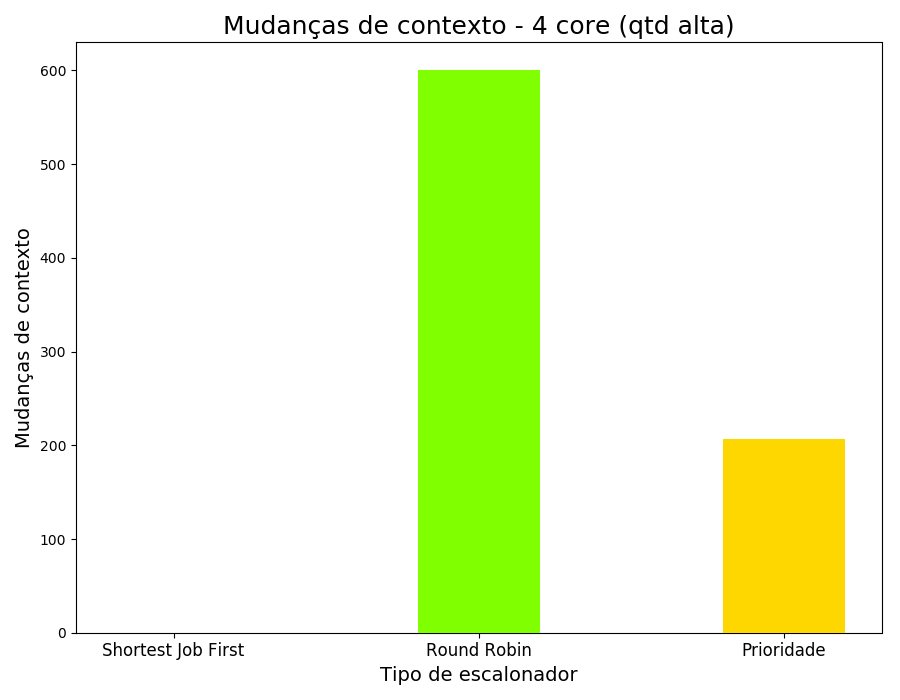
\includegraphics[scale=0.4]{ctx_long_4.png}
\end{figure}
\end{frame}

%------------------------------------------------
\subsection{Máquina B}

\begin{frame}
\frametitle{Cumprimento de deadlines (32 cores)}
\begin{figure}
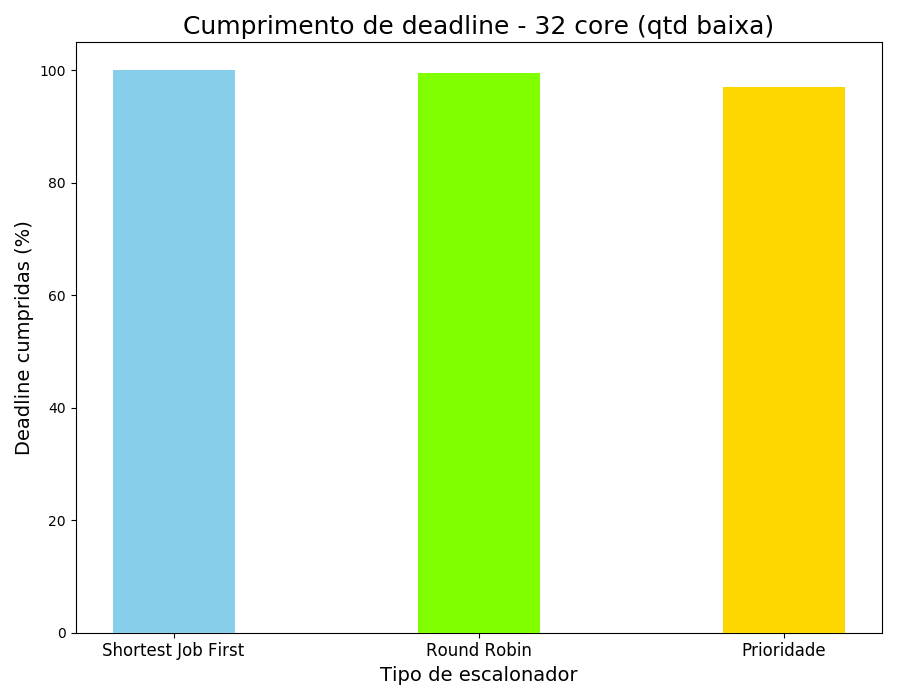
\includegraphics[scale=0.4]{deadline_small_32.png}
\end{figure}
\end{frame}

\begin{frame}
\frametitle{Cumprimento de deadlines (32 cores)}
\begin{figure}
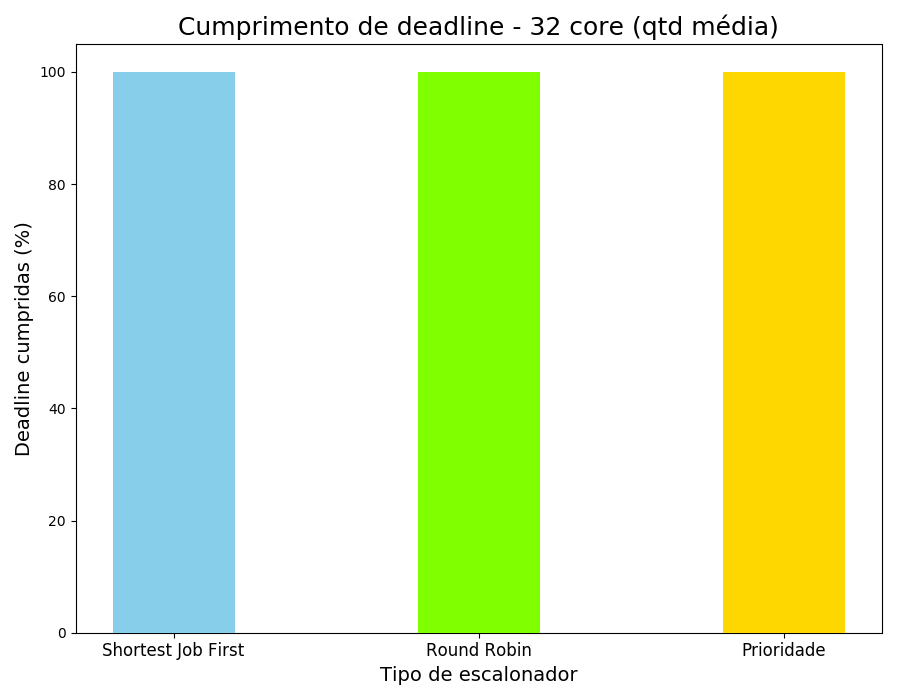
\includegraphics[scale=0.4]{deadline_med_32.png}
\end{figure}
\end{frame}

\begin{frame}
\frametitle{Cumprimento de deadlines (32 cores)}
\begin{figure}
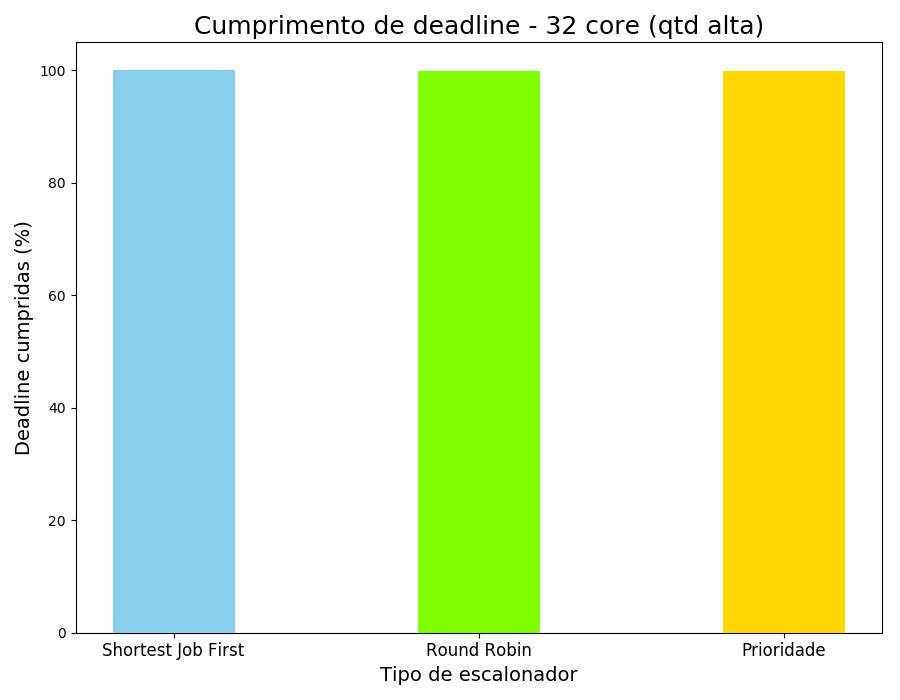
\includegraphics[scale=0.4]{deadline_long_32.png}
\end{figure}
\end{frame}

\begin{frame}
\frametitle{Mudanças de contexto (32 cores)}
\begin{figure}
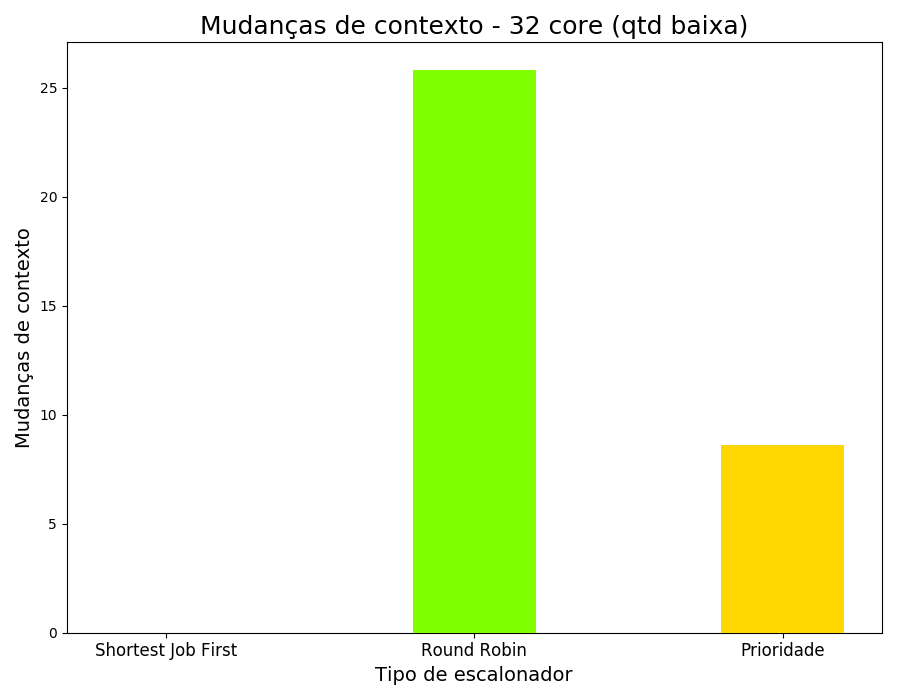
\includegraphics[scale=0.4]{ctx_small_32.png}
\end{figure}
\end{frame}

\begin{frame}
\frametitle{Mudanças de contexto (32 cores)}
\begin{figure}
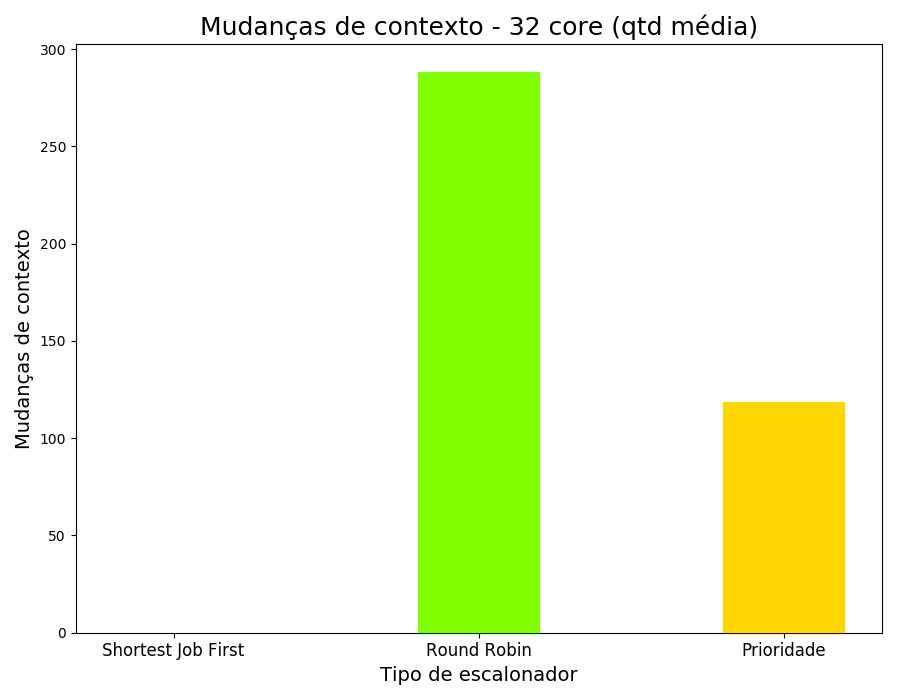
\includegraphics[scale=0.4]{ctx_med_32.png}
\end{figure}
\end{frame}

\begin{frame}
\frametitle{Mudanças de contexto (32 cores)}
\begin{figure}
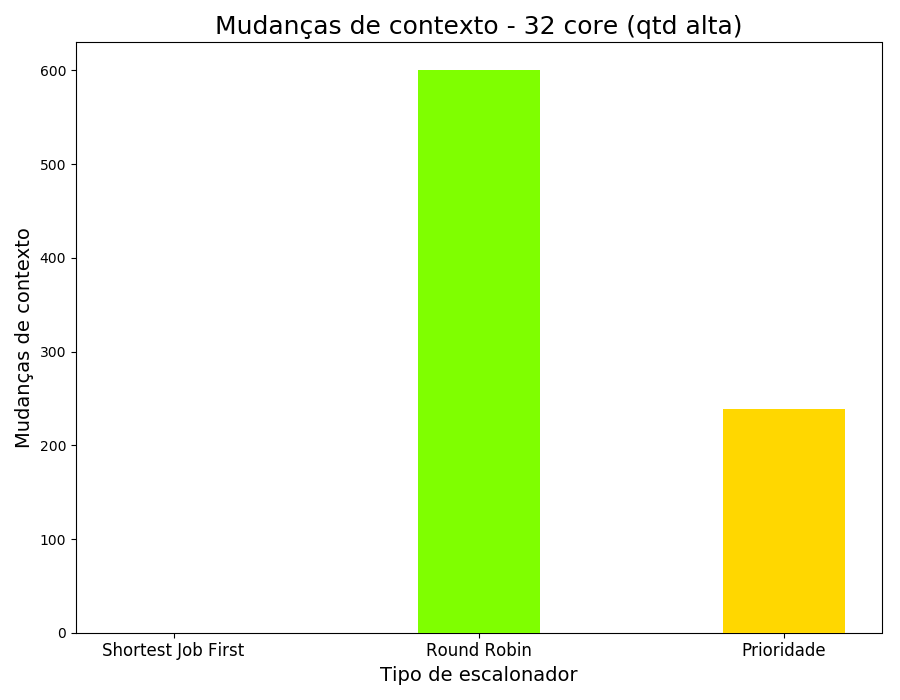
\includegraphics[scale=0.4]{ctx_long_32.png}
\end{figure}
\end{frame}

%------------------------------------------------
\section{Extras}
%------------------------------------------------

\begin{frame}
\begin{center}
\huge Extras
\end{center}
\end{frame}

\begin{frame}
\frametitle{Extra: Prioridade alternativa}
O multiplicador do quantum vai de 1 até 10. Inicialmente, a função que nos dava esse multiplicador era definida por:
$$Qmult(p) = -33\log_{10}\left(\frac{1}{1+e^{-\frac{p}{25}}}\right)$$
\begin{figure}
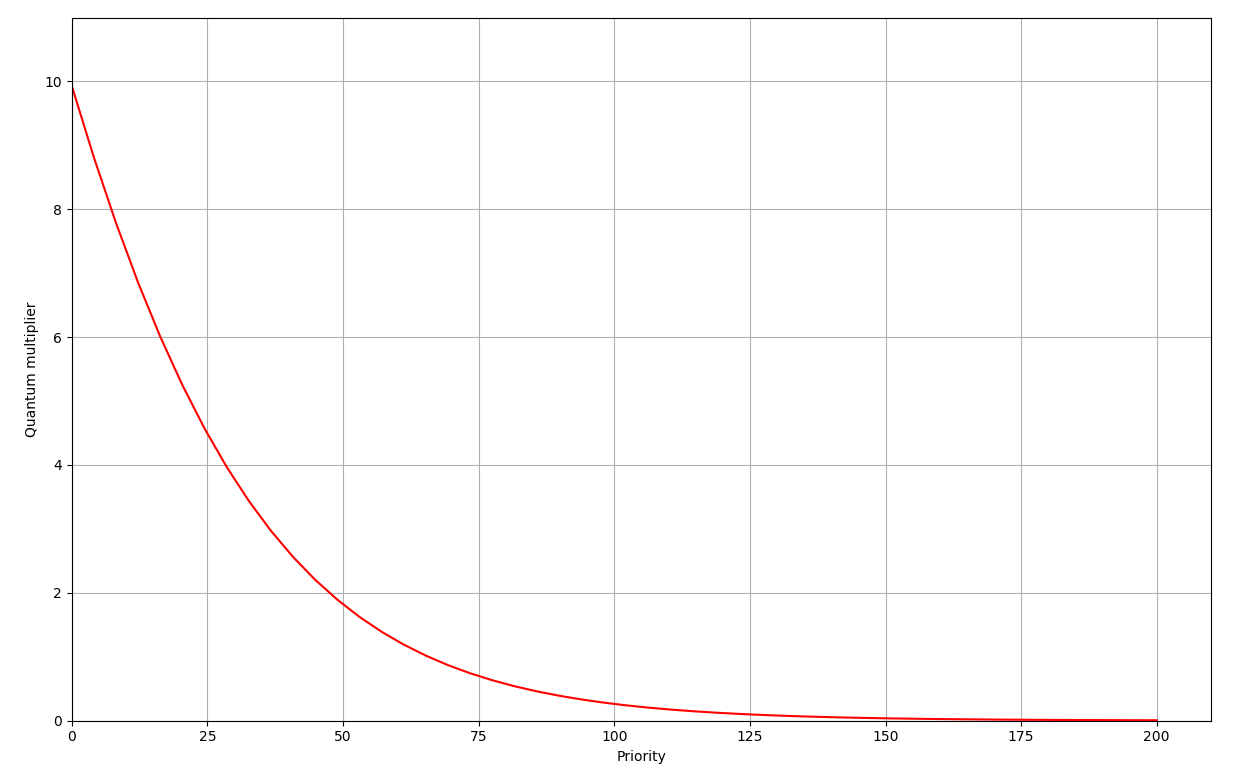
\includegraphics[scale=0.18]{sigmoidal.png}
\end{figure}
\end{frame}


\begin{frame}
\frametitle{Extra: Prioridade Alternativa}
Porém descartamos esse modelo e utilizamos o explicado anteriormente.
Algumas desvantagens que encontramos após rodar os testes:
\begin{itemize}
\item O multiplicador do quantum é estático (visando um ambiente interativo supomos que algo dinâmico se encaixava melhor)
\item Resultado com poucos processos era muito ruim
\item Resultado era bom com vários processos, mas no geral era pior que a outra forma
\end{itemize}
\end{frame}

\begin{frame}
\frametitle{Extra: Tempo médio de espera (4 cores)}
\begin{figure}
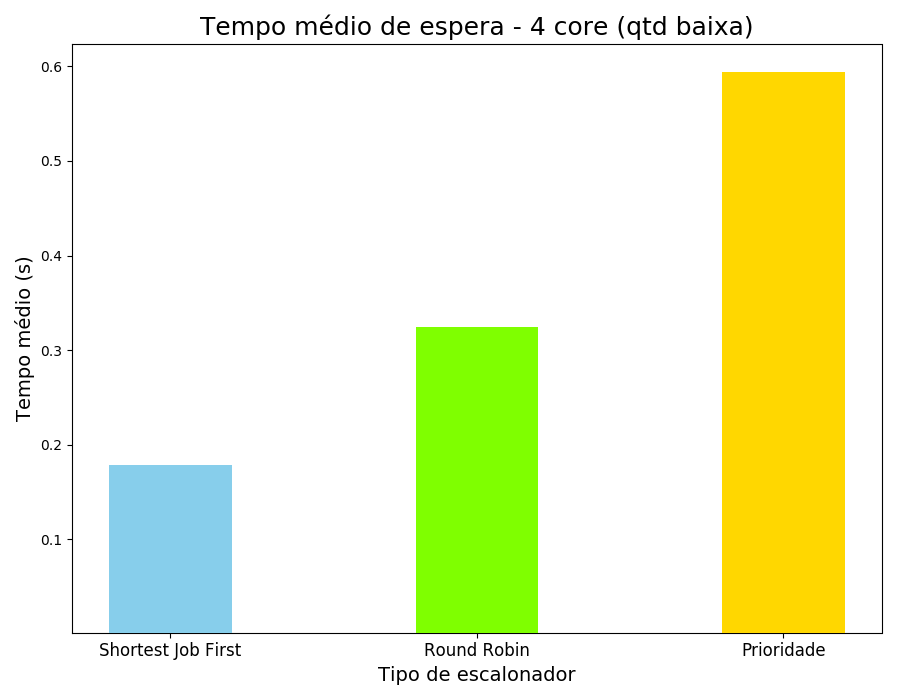
\includegraphics[scale=0.4]{avgwt_small_4.png}
\end{figure}
\end{frame}

\begin{frame}
\frametitle{Extra: Tempo médio de espera (4 cores)}
\begin{figure}
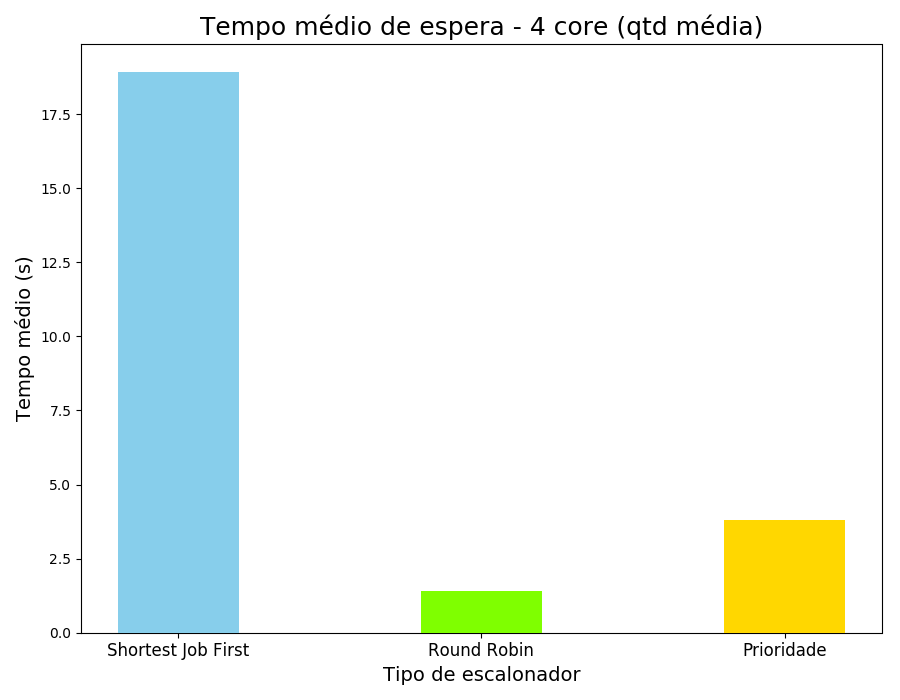
\includegraphics[scale=0.4]{avgwt_med_4.png}
\end{figure}
\end{frame}

\begin{frame}
\frametitle{Extra: Tempo médio de espera (4 cores)}
\begin{figure}
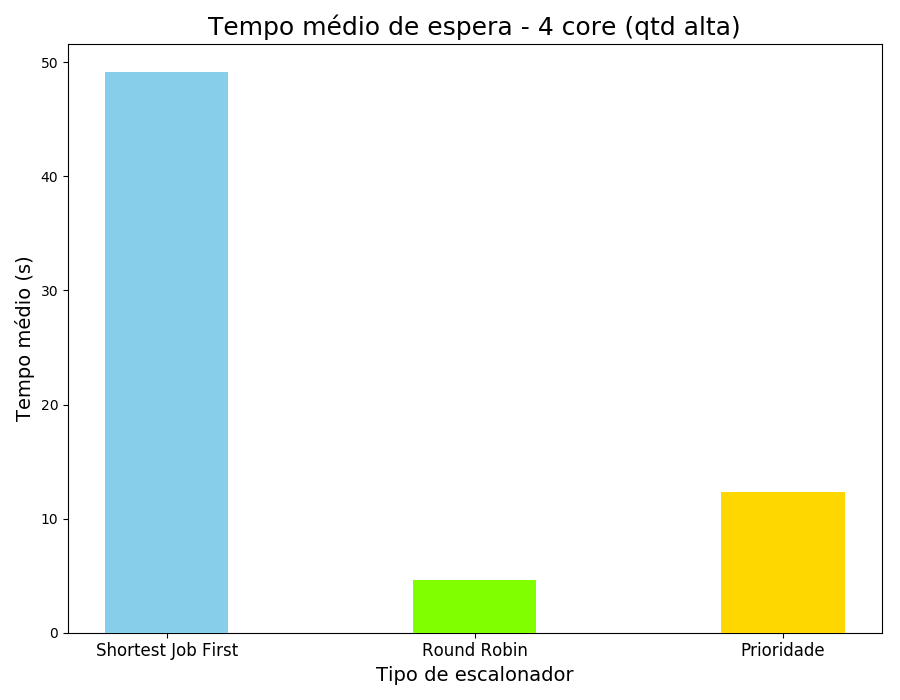
\includegraphics[scale=0.4]{avgwt_long_4.png}
\end{figure}
\end{frame}

\begin{frame}
\frametitle{Extra: Tempo médio de espera (32 cores)}
\begin{figure}
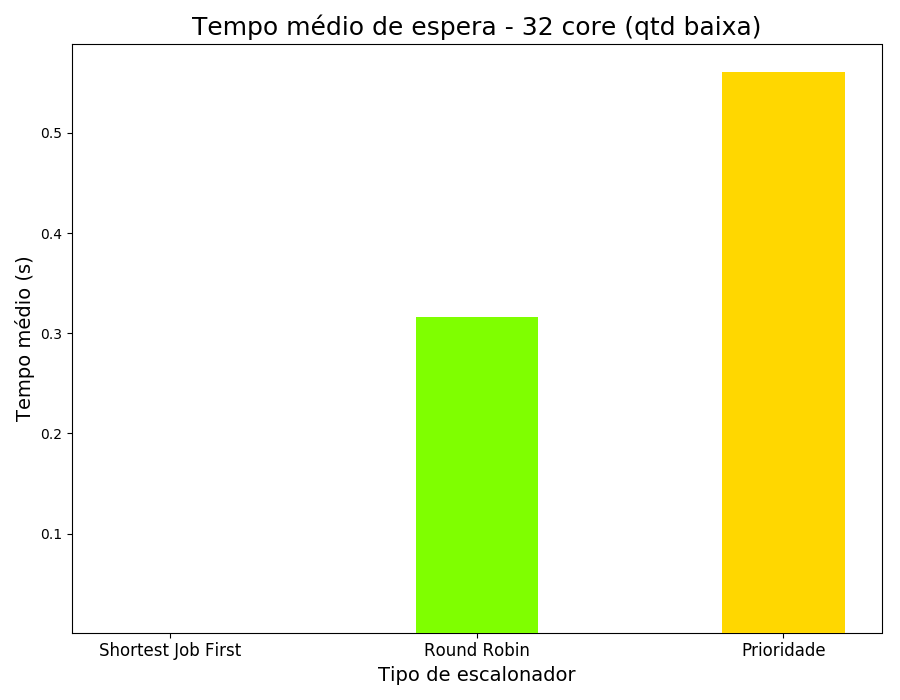
\includegraphics[scale=0.4]{avgwt_small_32.png}
\end{figure}
\end{frame}
\begin{frame}
\frametitle{Extra: Tempo médio de espera (32 cores)}
\begin{figure}
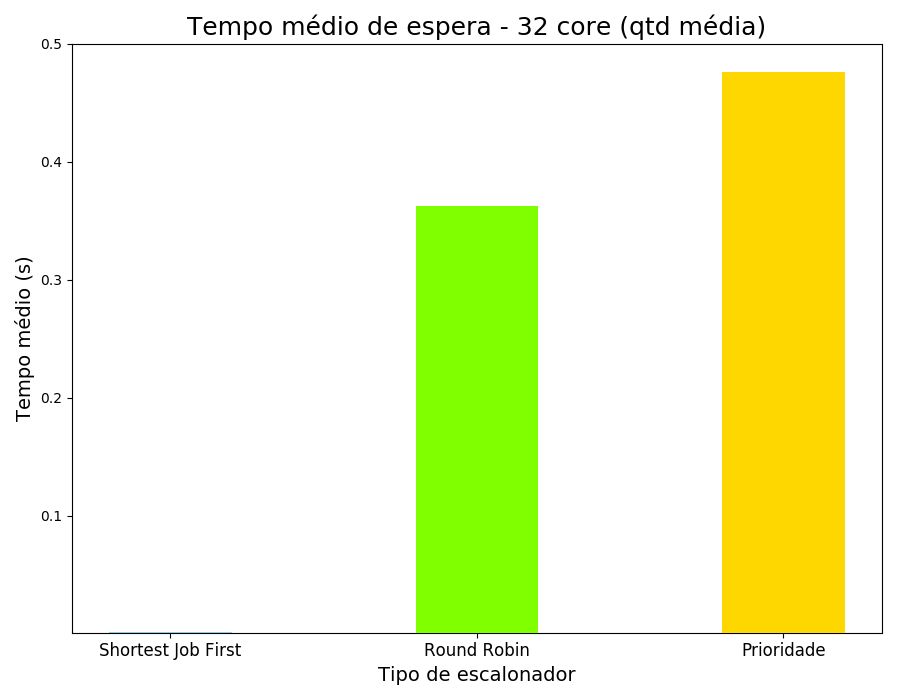
\includegraphics[scale=0.4]{avgwt_med_32.png}
\end{figure}
\end{frame}
\begin{frame}
\frametitle{Extra: Tempo médio de espera (32 cores)}
\begin{figure}
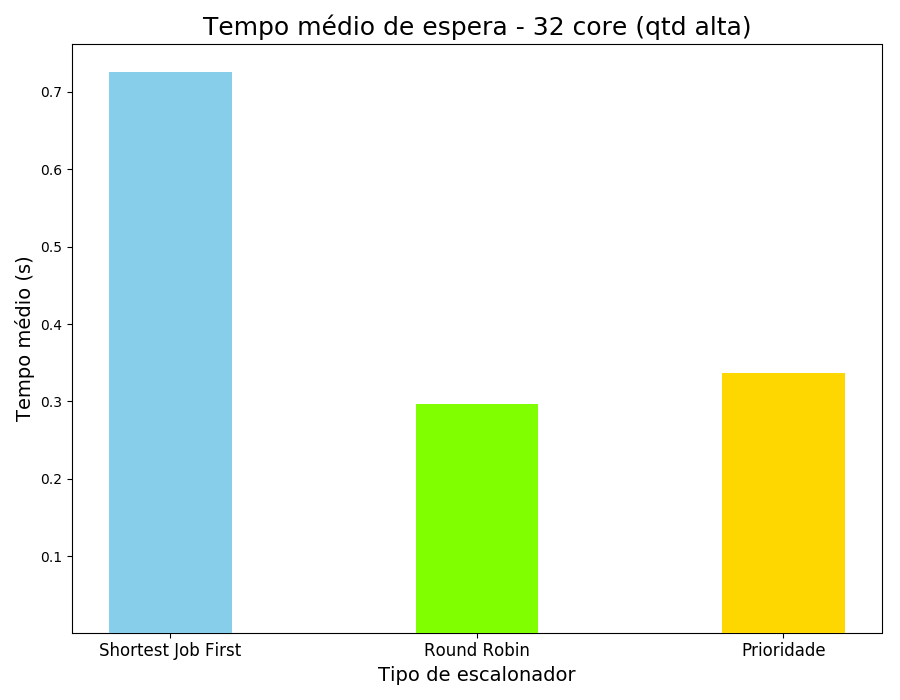
\includegraphics[scale=0.4]{avgwt_long_32.png}
\end{figure}
\end{frame}

\begin{frame}
\frametitle{Bibliografia}
\footnotesize {
\begin{thebibliography}{99} % Beamer does not support BibTeX so references must be inserted manually as below
\bibitem[Sedgewick, Robert and Wayne, Kevin]{p1} Sedgewick, Robert and Wayne, Kevin
\newblock Algorithms, 4th Edition.
\bibitem[Tanenbaum, Andrew S.]{p1} Tanenbaum, Andrew S.
\newblock Modern Operating Systems, 4th Edition.
\end{thebibliography}
}
	\end{frame}

\end{document}